\section{Design}
\label{sec:Design}

För att säkerhetssystemet ska fungera korrekt måste det klara av en mängd olika uppgifter. Bland annat: kontrollera om en dörr är öppen; avljuda larm; läsa och tolka värden från sensorer, och ta emot inmatning av användare. Systemet delas upp i moduler för att effektivt utföra de nödvändiga funktionerna. Detta underlättar även utvecklingen av projektet. En grafisk översikt av systemet visas nedan i figur \ref{fig:systemoversikt}. Rektanglarna är moduler och pilarna är de funktioner som anropas mellan dem.

\begin{figure}[H]
    \centering
    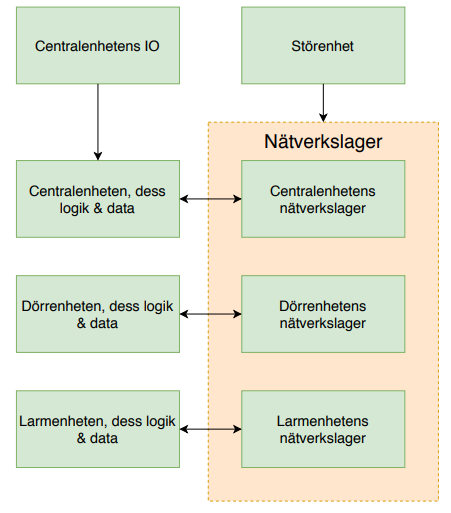
\includegraphics[scale=0.75]{dokumentation/projektplan/systemoversikt.png}
    \caption{Grafisk representation av systemet}
    \label{fig:systemoversikt}
\end{figure}


\subsection{Nätverklagret}
\label{sec:nätverklagretDE}
Ett CAN-protokoll designades för projektet. Den ram som designades syns
i figur \ref{fig:can_frame_own}. ID-fältet innehåller identifieringsinformation för meddelandet. RTR(Remote Transmission Request) innehåller information angående typen av ram. IDE(Identifier Extension) säger vilken typ av identifiering som ramen har. Längd ger längden på databufferten och databuffert
innehåller datan i fråga. Databufferten kan som längst vara åtta bytes lång. Utöver protokollet planerades också ett bibliotek för användandet av CAN. Ett sådant bibliotek hjälper uppfyllandet av krav ett under \ref{sec:kravspec}.

\begin{figure}[h]
    \centering
    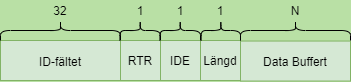
\includegraphics[scale=0.7]{dokumentation/projektrapport/IMAGES/can_frame_own.png}
    \caption{Den designade CAN-ramen}
    \label{fig:can_frame_own}
\end{figure}
\newpage

ID-fältet innehåller i sin tur data om meddelandet. Fältet visualiseras i figur \ref{fig:id_fält}. Samtliga sektioner i fältet beskrivs nedan:
\begin{description}
    \item[DIR] är meddelandets riktning. Är biten satt till noll är meddelandet ämnat till centralenheten. Är biten ett så är meddelandet från centralenheten.
    \item[Message ID] är meddelandets ID. Den säger vad det är för slags meddelande som skickats.
    \item[Node ID] har olika betydelser beroende på vad DIR-biten är satt till. Är DIR-biten satt till noll säger detta fält vilken enhet meddelandet är ämnat för. Men om DIR-biten är satt till ett beskriver fältet vilken nod meddelandet kom ifrån.
\end{description}
\begin{figure}[h]
    \centering
    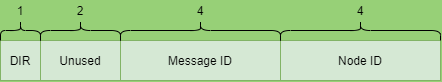
\includegraphics[scale=0.6]{dokumentation/projektrapport/IMAGES/protocol_new.png}
    \caption{CAN-ramens ID-fält, talen beskriver antalet bytes.}
    \label{fig:id_fält}
\end{figure}

Det fanns olika sorter av meddelanden som designades. Dessa syns tabell \ref{tab:msg_types} nedan. Genom att ha olika meddelandetyper blir det lättare att skriva hanteringsfunktioner för CAN-meddelanden då programmet utför rutiner baserat på typerna. Prioriteringen av diverse meddelandetyper är densamma som ordningen i tabellen, där högsta prioriteten är längst upp i tabellen.

\begin{table}[h]
    \caption{Alla typer av meddelanden. Högst prioritering längst upp i tabellen.}
    \begin{center}
     \begin{tabular}{ |c p{8cm}| }  
     \hline
     Typ & Betydelse  \\ [0.5ex] 
     \hline\hline
     Alarm & Säger åt larmenheten att den ska slå larm. \\ 
     \hline
     Ping & Ett vanligt pingmeddelande. När en periferienhet får ett pingmeddelande lägger enheten upp ett eget pingmeddelande på bussen som svar. \\
     \hline
     Konfigurering & Innehåller nya konfigurationer till en enhet. \\
     \hline
    \end{tabular}
    \end{center}
    \label{tab:msg_types}
\end{table}


\subsection{Centralenheten}
\label{sec:centralenhetenDE}
Om man sammanfattar centralenhetens uppgift ska den fungera som administratör för alla enheter. I \ref{sec:kravspec} nämns det att den ska lagra aktuell information om dessa och konfigurera om dem, men också att den ska larma om någon enhet blir frånkopplad. För att uppfylla dessa krav designades centralenhetens logik efter flödesschemat som visas i figur \ref{fig:centralflöd}. Datahanteringen utvecklades enligt kravspecifikation två, och logiken gällande enheterna enligt kravspecifikation fem.
\newline \newline
\begin{figure}[h]
    \centering
    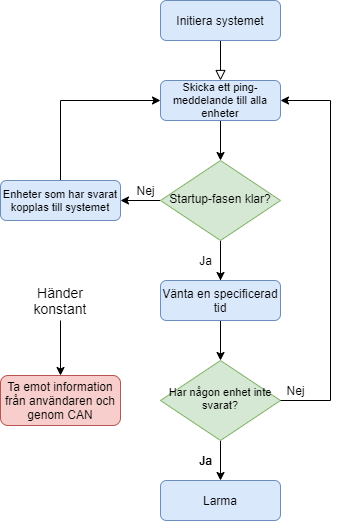
\includegraphics[scale=0.6]{dokumentation/projektrapport/IMAGES/centralenhet_flowchart.png}
    \caption{Flödesschema för centralenhetens logik}
    \label{fig:centralflöd}
\end{figure}
\newline \newline
I schemat beskrivs det att data konstant tas emot från användaren och CAN. Denna information handlar mest om de kopplade enheterna, och behöver lagras, både för användaren och systemet i helhet. Därför använder sig centralenheten av en lista, där varje plats i den innehåller information om en kopplad modul. Informationen inuti listan är en ''struct'', en datarepresentation av modulen. Dessa ''structs'' underlättar när specifik information ska hämtas gällande modulerna, och detta görs väldigt ofta i systemet.
\newline \newline
Schemat beskriver också centralenhetens logik; hur centralenheten kopplar enheter till systemet och detekterar om någon av dem blir frånkopplade. När uppstarts-fasen är klar är alla enheter anslutna till systemet, förutsatt att de svarade på ping-meddelandena som skickades. Centralenheten börjar då regelbundet skicka ut ping-meddelanden, väntar en specificerad tid, och undersöker om någon enhet inte har svarat i tid. Då larmar centralenheten globalt. Det här säkerhetsställer att inga delar av systemet kan kopplas bort utan att ett larm går.
\newline \newline
Uppstarts-fasen är designad med avseende på modularitetskravet (krav åtta). Systemet är inte ''låst'' till en speciell uppsättning enheter; alla som svarar på centralenhetens ping-meddelanden blir anslutna. Användningen av listan med ''structs'' möjliggör denna process. Teoretiskt sett kan en godtycklig mängd enheter av varierande typ kopplas till systemet. Detta underlättar också för användaren - systemets delar är anslutna så fort uppstart-fasen är färdig, utan någon konfiguration.

\subsection{Centralenhetens IO}
\label{sec:centralenhetIODE}
% används för att ta emot en kod användaren har slagit in för att stänga av larmet vilket sedan vidarebefordras till centralenheten som verifierar koden. USART används för att ge kommandon och konfigurera moduler. USART används även som en utport där programmet kan skriva ut statusmeddelande för att simplifiera debugging-processen.
%\newline\newline
Centralenheten IO består av en knappsats och USART. IO funktionerna för dessa utvecklades enligt kravspecifikation \ref{itm:krav3}, \ref{itm:krav4} och \ref{itm:krav7} (se \ref{sec:kravspec}). Därmed är knappsatsen designad för ta emot en sifferkod samt att lagra den för centralenhetens användning. USART utformades dels för att skicka utmatningar från centralenheten som presenteras för användaren. USART designades även för att ta emot inmatningar från användaren vilket tillåter konfigurationer och status meddelanden. Konfigurationerna sker via olika kommandon som användaren kan skriva in i USART. \\

Både knappsatsen och USART utvecklades för att inte avbryta programmet, vilket tillåter ett kontinuerligt program där alla funktioner kan köras vid alla tidpunkter. Detta krävs för en korrekt fungerande centralenhet då ping meddelanden måste mottas och hanteras konstant. (\ref{sec:centralenhetenDE}, figur \ref{fig:centralflöd}).

% Design IO = motivera och förklara grundläggande USART och knappsats funktioner, dvs bufferten, referera till centralenheten + krav för varför det behövs.  Systemet skall kunna hantera inmatningar ifrån USART och keypad samtidigt som den kör.

% Teknisk bakgrund IO = implementation av USART, säg buffertsystem, anledningen till buffersystemet finns redan.  

\subsection{Dörrenheten}
\label{sec:dörrenhetenDE} % cant write des:door, maybe try sec:doorDE
Säkerhetssystemet designades för att kunna hantera flera dörrar. Ett alternativ hade varit att ha en dörr per MD407-kort. Dock, eftersom att ett MD407-kort har förmågan att hantera ett flertal dörrsensorer utnyttjas det. Då blir det enklare samt effektivare att koppla upp ett större antal dörrar. Antalet uppkopplade dörrar bestäms i centralenheten. Varje dörr förses med ett unikt ID för att kunna skilja dem åt samt konfigurera dem separat. Konfigurationen sker genom att det skickas och mottages meddelanden över CAN med hjälp av CAN-protokollet i enlighet med krav ett och fyra (\ref{sec:kravspec}).
\newline\newline
En dörrs larmfunktion kan aktiveras och avaktiveras. En avaktiverad dörr signaleras med en grön diod. 
Enligt kravspecifikationen har dörrenheten både lokalt och globalt larm. 
Det lokala larmet, en röd diod, går efter dörren varit öppen längre än en given tid. 
Det används för att inte larma globalt i onödan. 
Exempelvis i fallet att dörren öppnas av misstag och sedan omedelbart stängs igen. 
Meddelande om globalt larm skickas till centralenheten då dörren varit öppen längre än en ytterligare angiven tidsgräns. 
Centralenheten avgör sedan hurvida larmenheten ska tjuta. Hur lång tid innan globalt samt lokalt larm ges kan konfigureras via CAN.

\subsection{Larmenheten}
\label{sec:LarmenhetenDE}
Larmenhetens huvudsakliga uppgift är att utlösa ett ljudbaserat larm om rätt krav möts. Dessa krav är antingen att centralenheten skickar ett meddelande över CAN om att utlösa larmet eller att larmenhetens sensorer har mätt ett visst värde. Sensorerna består utav en vibrationssensor  och en avståndssensor som skickar mätdata till larmenheten.
\newline\newline
Kommunikationen från Centralenheten via CAN-bussen har högsta prioritet eftersom även centralenheten snabbt måste kunna utlösa larmet vid behov. Det har ordnats genom att mottagna meddelanden skapar avbrott i systemet. Avbrottshanteraren för vidare meddelandet till en hanteringsfunktion beroende på vilken typ av meddelande det är. De meddelandetyper som hanteras är konfigureringsmeddelanden enligt krav fyra (\ref{sec:kravspec}), meddelanden för att växla av/på larmet och pingmeddelanden. 
\newline\newline
Enligt krav sex (\ref{sec:kravspec}) har larmenheten en utbyggnad i form av ett lokalt larm. Detta lokala larm består av en lampa som tänds när någon eller något närmar sig avståndssensorn. Syftet för utbyggnaden är att det ska avråda folk från handlingar som skulle leda till ett globalt larm. \\

\subsection{Störenheten}
\label{sec:störenhetenDE}
Störenheten utvecklades för att simulera en defekt periferienhet genom att skicka stora mängder data på CAN-nätverket. Enheten kan skicka faktiska meddelanden eller slumpad data. Förmågan att skicka båda typer utvecklades för att ha möjlighet att testa en bredare mängd problem som skulle kunna uppstå.

%referera till detta?%
\iffalse
\begin{enumerate}
    \item Enheterna ska kunna kommunicera genom CAN-bussen på ett konsekvent sätt.
    \label{itm:krav1}
    
    \item Centralenheten ska lagra aktuell information om alla enheter.
    \label{itm:krav2}
    
    \item Centralenheten ska presentera den viktigaste informationen för användaren genom USART.
    \label{itm:krav3}
    
    \item Periferienheterna ska vara konfigurerbara genom USART.
    \label{itm:krav4}
    
    \item Centralenheten ska larma ifall någon periferienhet går sönder eller blir frånkopplad.
    \label{itm:krav5}
    
    \item Periferienheterna ska tillämpa ett lokalt larm om sensorer blir triggade, och larma globalt om det behövs.
    \label{itm:krav6}
    
    \item Om larmet har gått kan det avaktiveras från centralenheten genom att en kod matas in på en knappsats.
    \label{itm:krav7}
    
\end{enumerate}
\fi